\section{User Evaluation}
\begin{figure}[t!]
    \centering
    \begin{subfigure}[t]{1\columnwidth}
        \centering
        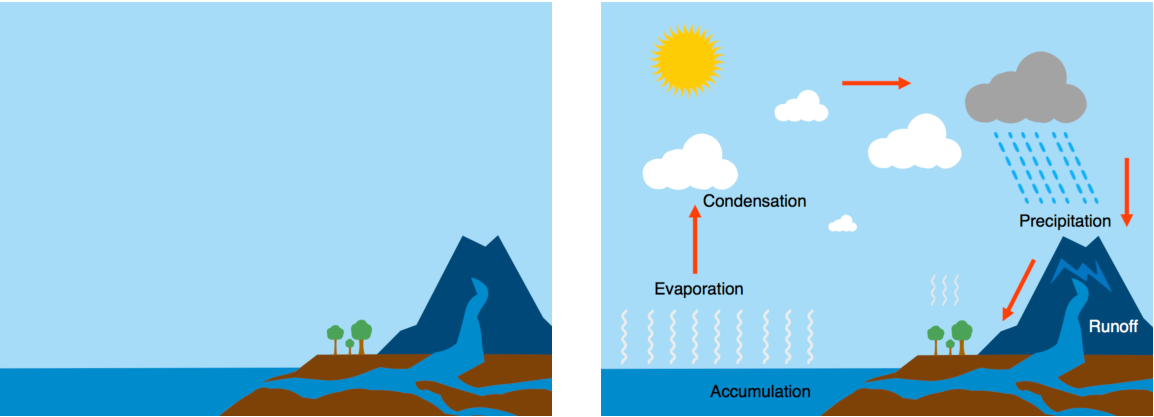
\includegraphics[width=1\columnwidth]{figures/watercycle}
        \caption{\textit{WaterCycle} slide background (left) and foreground (right)}
    \end{subfigure}
    ~ 
    \begin{subfigure}[t]{0.48\columnwidth}
        \centering
        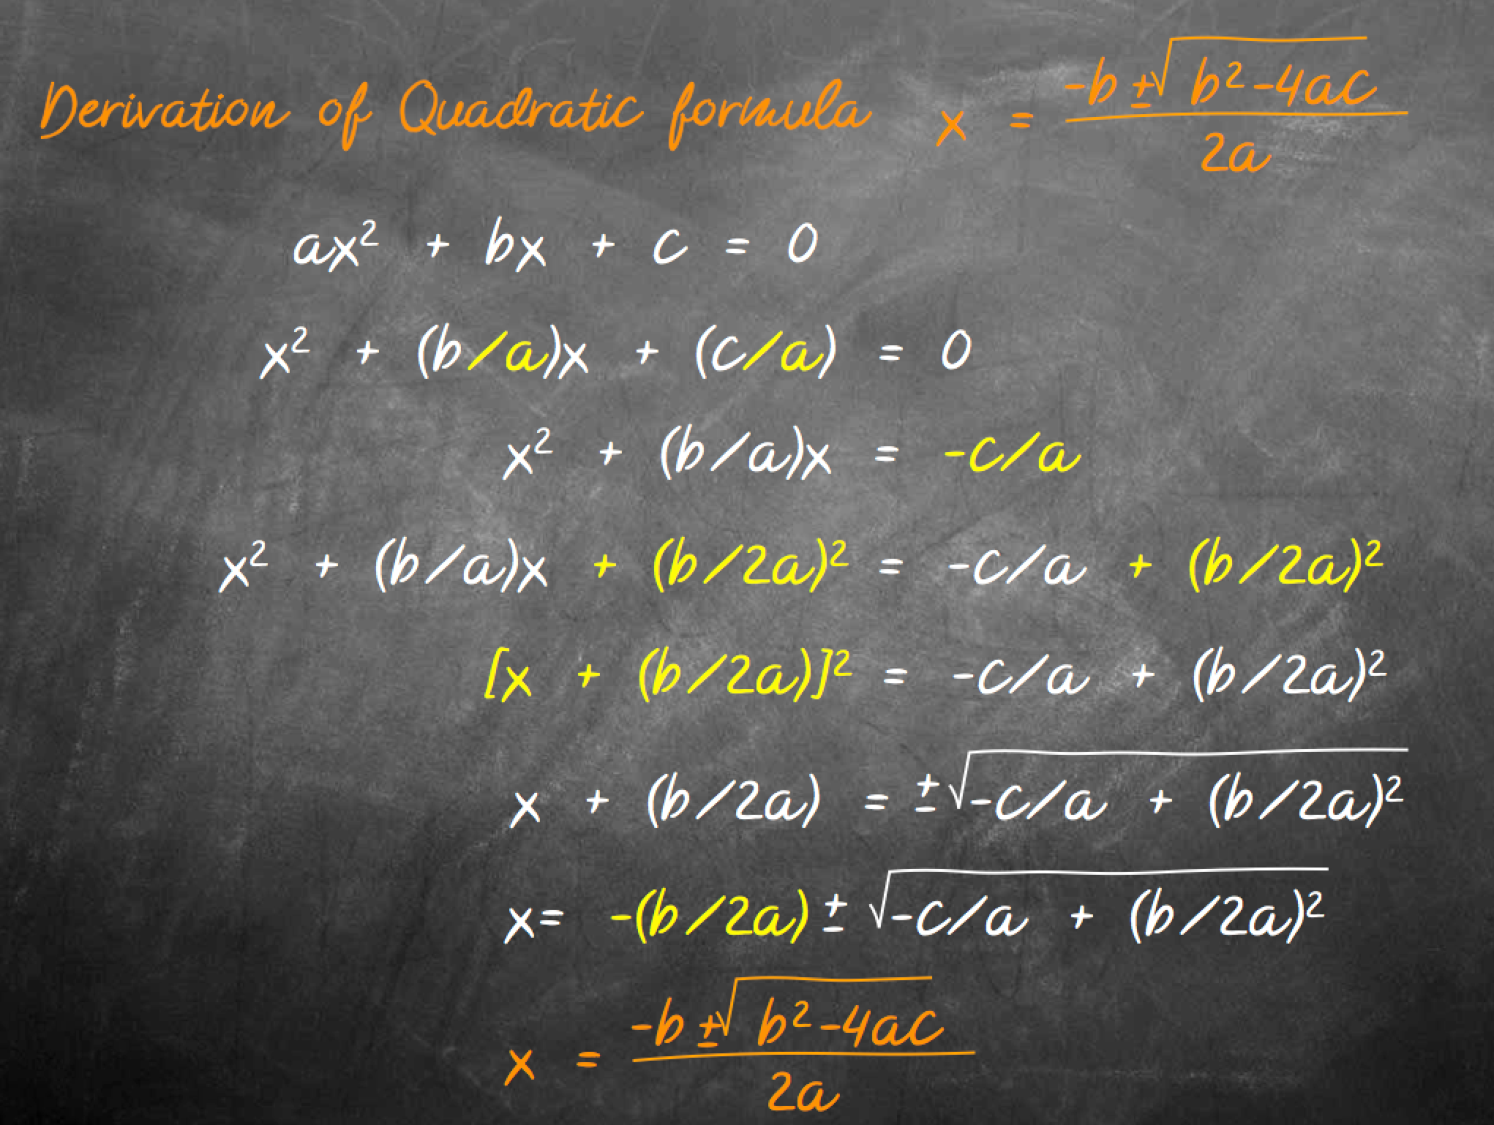
\includegraphics[width=1\columnwidth]{figures/quadformula}
        \caption{\textit{Derivation} slide}
    \end{subfigure}  
    ~
    \begin{subfigure}[t]{0.48\columnwidth}
        \centering
        
\includegraphics[width=1\columnwidth]{figures/tools}
        \caption{\textit{BulletPoints} slide}
    \end{subfigure}  
    \caption{Evaluation slides}
    \label{fig:studyslides}
\end{figure}

We evaluate \interface\ from the perspective of presenters and the audience. We assess the ease of use of the interface from the presenters' point of view, and rate the presentation quality from both the presenters' and the audiences' perspective.

%\wil{If we have time, it could be useful to include even an informal
%  evaluation of the space manipulation features. Maybe just give users
%  a script that includes explicit ``improvisations'' beyond the
%  prepared content and ask for qualitative feedback?}

%\val{Explain that we specifically focus on the delivery stage (vs. authoring).}
To better understand the benefits of our interface, we compared \interface\ against two baselines. The first baseline (\textit{BaselinePPT}) represents conventional electronic slide tools.
%
We use Microsoft PowerPoint and allow presenters to apply animation effects (but no inking) during the presentation.
%
The second baseline (\textit{BaselineInk}) represents standard ``blackboard-style'' presentation tools that allows users to ink in real-time during the presentation.
%
For this condition, we also use Microsoft PowerPoint but only allow users to pre-author and deliver content via inking.

We hypothesized that different types of content would lend themselves to different presentation styles. We compare three different types of content: (1) a text-centered slide, explaining the derivation of the quadratic formula \textit{(Derivation)}, (2) a diagram-centered slide, describing the hydrologic cycle  \textit{(WaterDiagram)}, and (3) a typical PPT style slide with bullet points and images listing different carpentry tools \textit{(BulletPoints)}. Using PowerPoint, we pre-authored a single page slide for each of these content types. (Figure~\ref{fig:studyslides}) 
%

To reduce the preparation effort for all three presentation tool conditions, we separated each slide into foreground and background elements, which are shown in our supplemental materials. For the \textit{BaselinPPT} condition, we leave the individual PowerPoint elements (e.g., arrows, text boxes containing individual lines of equations, images) without further grouping them to make it easier for users to author fine-grained animations. 
%
%\val{Figure of three slides, including explanation of background foreground}
%\wil{I edited above. Is this correct?}

\subsection{Study 1: Presenter Perspective}
In our first study, we asked participants to present each of the three content types using the three different presentation tool conditions. 
%
For each content type, participants were given the pre-authored, pre-segmented slide. 
They received verbal and written explanations of the material, and a printout of the complete slide contents (both foreground and background layers). They were given time to familiarize themselves with this material and to set up the slide before the presentation.
%
In the \textit{BaselinePPT} condition, participants could add animation effects to reveal or emphasize the foreground elements. For the \textit{BaselineInk} condition, the slide only contained background elements. Participants were free to write additional content into the slide as part of their set up, which is analogous to blackboard lecturers writing on the board before class. For \interface, participants could also write additional content on top of the background, or they could choose to make some of the foreground elements visible (effectively moving those elements into the background layer). \val{We only evaluated the ink to reveal and ink to annotate.}

After the setup phase, participants used one of the three tool conditions to deliver the presentation. 
%
To simulate a real presentation with an audience, participants were asked to pretend that their presentation was being broadcast live as a webcast. At the end of each trial, we showed the user a screen recording of their presentation and asked them to self-rate their own presentation, this time pretending that they were students trying to learn the subject. Presenters also completed a questionnaire where they rated how easy it was to prepare and deliver presentations using each of the tools. All ratings were done on a 5-point Likert scale.

We used a within-subject design, where each participant delivered presentations on each interface. We kept the task order fixed and counter-balanced the order of the presentation tools to obtain an equal distribution of task-tool pairs.
%
There were 12 participants in total (ages 21 to 31), all of whom were familiar with the PowerPoint interface. 

\subsection{Study 2: Audience Perspective}
In our second study, we recruited a separate set of participants to vote on presentations delivered using each interface.
%
While we considered comparing the output presentations from the first study, we found that there was too much variation in quality between the results. Since presenters were not forced to follow fixed scripts, there were significant differences in length and detail. In addition, the presenters spoke with varying levels of enunciation and enthusiasm (not to mention different accents).
%
Thus, we ourselves produced a new set of more comparable presentations
using the slides from the first study.
%
To make the comparison as fair as possible, we used a fixed script for each content type.
We also analyzed the output presentations from the first study, and used them as a reference when creating our own versions. 
%
For example, for the BaselinePPT condition, we reproduced the granularity and order of animations that we observed in the user-created presentations.
%a
In the BaselineInk condition, we followed the typical ordering of the inked contents and chose similar ink colors. We also recorded the presentations so that the silent pauses in between inking periods were similar (or shorter) than those produced in the first study. 
%
Finally, for \interface, we used a similar reveal order, combination of slow tracing versus fast scribbling, and on-the-fly ink annotations as most participants. 
%
In general, presenters from the first study employed similar approaches so it was straight-forward to extract common qualities. For the few cases, where participants varied in their approach, we selected an approach that we deemed to produce better quality (e.g., finer-grained animations, use of different ink colors). The final recordings of the presentations from both studies are included in the supplementary material. 

We recruited 36 participants to rate the presentations. For each content type, participants watched recordings of three presentations delivered using each interface, and voted for the most engaging presentation. 














